%\documentclass[notes=show,xcolor=table]{beamer}
\documentclass[xcolor=table]{beamer}
% german and utf8
\usepackage[ngerman]{babel}
\usepackage[utf8]{inputenc}
\usepackage{listings}



\usepackage{lmodern}

\usepackage{graphicx, hyperref}
% Das Paket lmodern erspart die folgenden Warnungen:
% LaTeX Font Warning: Font shape `OT1/cmss/m/n' in size <4> not available
% (Font)              size <5> substituted on input line 22.
% LaTeX Font Warning: Size substitutions with differences
% (Font)              up to 1.0pt have occurred.
 
% beamer style 
%\usepackage{beamerthemeshadow}
\usetheme{Frankfurt}  
\usecolortheme[named=blue]{structure}


\setbeamertemplate{footline}{
	\leavevmode%
	\hbox{%
		\begin{beamercolorbox}[wd=.15\paperwidth,ht=2.25ex,dp=1ex,center]{date in head/foot}%
			\usebeamerfont{date in head/foot}\insertshortdate{}
		\end{beamercolorbox}%
%		\begin{beamercolorbox}[wd=.2\paperwidth,ht=2.25ex,dp=1ex,center]{author in head/foot}%
%			\usebeamerfont{author in head/foot}\insertshortauthor%~~(\insertshortinstitute)
%		\end{beamercolorbox}%
		\begin{beamercolorbox}[wd=.7\paperwidth,ht=2.25ex,dp=1ex,center]{title in head/foot}%
			\usebeamerfont{title in head/foot}\insertshorttitle
		\end{beamercolorbox}%
		\begin{beamercolorbox}[wd=.15\paperwidth,ht=2.25ex,dp=1ex,right]{date in head/foot}%
			\usebeamerfont{date in head/foot}\insertframenumber{} / \inserttotalframenumber{}
		\end{beamercolorbox}%
	}%
	\vskip0pt%
}

% allow colored tables
% http://tex.stackexchange.com/questions/68371/how-to-highlight-table-rows-by-colors-in-beamer
% for a more sophisticated solution see http://tex.stackexchange.com/a/18430/10327
\rowcolors{1}{gray!30}{gray!10}

\makeatletter
\def\rowcolor{\noalign{\ifnum0=`}\fi\bmr@rowcolor}
\newcommand<>{\bmr@rowcolor}{%
	\alt#1%
		{\global\let\CT@do@color\CT@@do@color\@ifnextchar[\CT@rowa\CT@rowb}%
		{\ifnum0=`{\fi}\@gooble@rowcolor}%
}

\newcommand{\@gooble@rowcolor}[2][]{\@gooble@rowcolor@}
\newcommand{\@gooble@rowcolor@}[1][]{\@gooble@rowcolor@@}
\newcommand{\@gooble@rowcolor@@}[1][]{\ignorespaces}
\makeatother

\usepackage{color, colortbl}
\definecolor{LRed}{rgb}{1,.8,.8}
\definecolor{MRed}{rgb}{1,.6,.6}
\definecolor{HRed}{rgb}{1,.2,.2}

% speech bubbles
% http://tex.stackexchange.com/questions/38805/simple-speech-bubbles-arrows-or-balloon-like-shapes-in-beamer
\usepackage{tikz}
\usetikzlibrary{calc,shapes.callouts,shapes.arrows}
% usage: \arrowthis{There is}{Corot}
\newcommand{\arrowthis}[2]{
	\tikz[remember picture,baseline]{\node[anchor=base,inner sep=0,outer sep=0]%
		(#1) {\underline{#1}};
		\node[overlay,single arrow,draw=none,fill=red!50,anchor=tip,rotate=60] 
	at (#1.south) {#2};}%
}%
\newcommand{\speechthis}[2]{
	\tikz[remember picture,baseline]{\node[anchor=base,inner sep=0,outer sep=0]%
		(#1) {\underline{#1}};\node[overlay,ellipse callout,fill=blue!50] 
	at ($(#1.north)+(-.5cm,0.8cm)$) {#2};}%
}%
\newcommand{\bubblethis}[2]{
	\tikz[remember picture,baseline]{\node[anchor=base,inner sep=0,outer sep=0]%
		(#1) {\underline{#1}};\node[overlay,cloud callout,callout relative pointer={(0.2cm,-0.7cm)},%
	aspect=2.5,fill=yellow!90] at ($(#1.north)+(-0.5cm,1.6cm)$) {#2};}%
}%
\newcommand{\pointthis}[2]{
	\tikz[remember picture,baseline]{\node[anchor=base,inner sep=0,outer sep=0]%
		(#1) {\underline{#1}};\node[overlay,rectangle callout,%
	callout relative pointer={(0.2cm,0.7cm)},fill=green!50] at ($(#1.north)+(-.5cm,-1.4cm)$) {#2};}%
}%


% allow strikethrough with \sout
% http://tex.stackexchange.com/questions/23711/strikethrough-text
%\usepackage{ulem}

% multimedia
% http://mo.mathematik.uni-stuttgart.de/inhalt/aussage/aussage1325/
% http://tex.stackexchange.com/questions/429/animation-in-pdf-presentations-without-adobe-reader
% http://www.ctan.org/pkg/animate

% againframe 
% http://stackoverflow.com/questions/171708/latex-beamer-package-change-frame-title-in-againframe
% http://tex.stackexchange.com/questions/31031/beamer-repeat-variations-of-a-frame

% todo notes
% http://tex.stackexchange.com/questions/11177/how-to-write-hidden-notes-in-a-latex-file

% http://www.texample.net/tikz/examples/feature/overlays/
% http://tex.stackexchange.com/questions/14769/add-more-anchors-to-standard-tikz-nodes

%\beamersetuncovermixins{\opaqueness<1>{25}}{\opaqueness<2->{15}}
% sorgt dafuer das die Elemente die erst noch (zukuenftig) kommen nur schwach angedeutet erscheinen
% klappt auch bei Tabellen, wenn teTeX verwendet wird\ldots

% http://tex.stackexchange.com/questions/16357/how-can-i-position-an-image-in-an-arbitrary-position-in-beamer
\usepackage{tikz}
%\usetikzlibrary{calc, trees, positioning, arrows, shapes, shapes.multipart, shadows, matrix, decorations.pathreplacing, decorations.pathmorphing}
\usetikzlibrary{arrows}%, shapes}%, shapes.multipart}%, automata}
\tikzset{
  every boverlay node/.style={
    draw=black,fill=white,rounded corners,anchor=north west,
  },
}
\tikzset{
  every toverlay node/.style={
	anchor=center
  },
}
\tikzset{
  every overlay node/.style={
    draw=white,fill=white,rounded corners,anchor=north west,
  },
}
% Usage:
% \tikzoverlay at (-1cm,-5cm) {content};%
% or
% \tikzoverlay[text width=5cm] at (-1cm,-5cm) {content};%
\def\tikzboverlay{% A bordered overlay
   \tikz[baseline,overlay]\node[every boverlay node]
}%
\def\tikztoverlay{% A transparent overlay
   \tikz[baseline,overlay]\node[every toverlay node]
}%
\def\tikzoverlay{% A non-transparent unbordered overlay
   \tikz[baseline,overlay]\node[every overlay node]
}%



\title{Knowledge Resources}
\author{Stefan Junghans\and\\Mitja Richter}
\date{June 11 2014}

\begin{document}

	\begin{frame}
		\titlepage
	\end{frame}

	\begin{frame}
		\frametitle{Table of Contents}
		\tableofcontents
	\end{frame}


	
	\section{Definition}

\begin{frame}
\frametitle{Definition}
\begin{itemize}
  \item Knowledge-based system
  \begin{itemize}
    \item Reasoner
    \item Knowledge Base
  \end{itemize}
  \item[]
	\item A database used for knowledge sharing and management
	\item Promotes the collection, organization and retrieval of knowledge
\end{itemize}

\end{frame}

\begin{frame}
\frametitle{Definition}

\begin{itemize}
    \item Human-readable
    \begin{itemize}
      \item Documents, Manuals, FAQs, \ldots
      \item Wikipedia, transfermarkt.de, \ldots
    \end{itemize}
    \item[]
    \item Machine-readable
    \begin{itemize}
      \item System-readable forms
      \item Ontologies
      \item less interactive than human-readable forms
      \item essential to the semantic web
      \item DBpedia, Freebase, \ldots
    \end{itemize}
    
\end{itemize}

\end{frame}

	\AtBeginSection[]{
		\begin{frame}
% 			\frametitle{Table of Contents}
			\tableofcontents[currentsection] 
		\end{frame}
	}
	
	\section{WordNet}
\begin{frame}
\frametitle{WordNet}

\includegraphics[scale=0.35]{img/wordnet_logo.png}
\begin{itemize}
\item development started 1985
\item lexical database for English language
\item covers most English nouns, verbs, adjectives, adverbs
\item used in many applications (retrieval, translation)
\item two kinds of semantic relations
\end{itemize}
% which means it labels concepts to words
\end{frame}

\begin{frame}
\begin{itemize}
\frametitle{Synsets - Lexical (word-word) relation}
\item words are grouped into synonym sets - synsets
\item sysnsets are the basic unit of meaning
\item 120,000 synsets
\item Synonym, Antonymy, Gradation
\end{itemize}
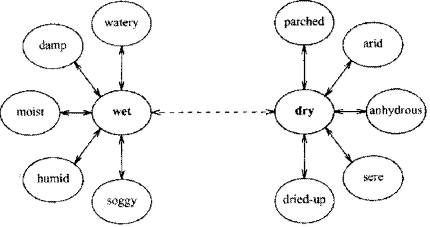
\includegraphics[scale=0.55]{img/wordnet-syn.png}
% Gradation in this context means it's related to all comparative words, for example wet, wetter, the wettest
\end{frame}

\begin{frame}
\begin{itemize}
\frametitle{Homonyms}
\item Homonyms are represented in several Synsets
\end{itemize}
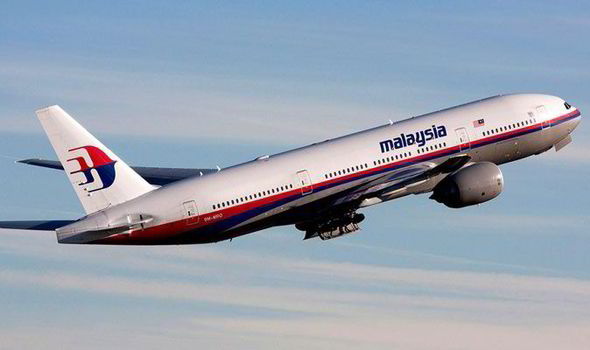
\includegraphics[scale=0.25]{img/plane2.jpg}
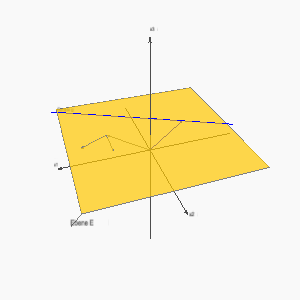
\includegraphics[scale=0.29]{img/wordnet_plane1.png}
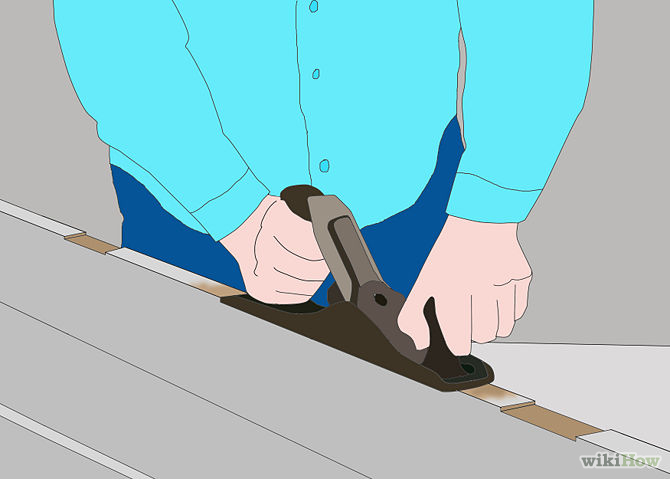
\includegraphics[scale=0.18]{img/plane3.jpg}
\end{frame}

\begin{frame}
\begin{minipage}{0.40\textwidth}
\begin{itemize}
\frametitle{Linking between Synsets - Conceptual (concept-concept) relation}
\item Synsets are linked by
\begin{itemize}
\item Hypernymy / Hyponymy
\item Meronymy / Holonymy 
\item Entailment 
\item Troponymy
\end{itemize}
\end{itemize}
\end{minipage}
\begin{minipage}{0.5\textwidth}
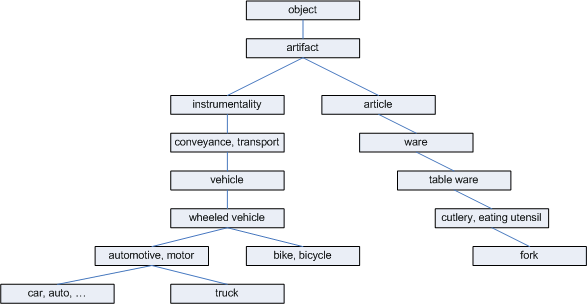
\includegraphics[scale=0.33]{img/wordnet_hyponym.png}
\end{minipage}
\end{frame}

\begin{frame}
\frametitle{Hypernym / Hyponym}
\begin{minipage}{0.5\textwidth}
\begin{itemize}
\item A truck (Hyponym) is a kind of car (Hypernym)
\item denotes more or less general concepts
\item transitive
\item experiments indicate knowledge about concepts is stored at superordinate (Hypernym) nodes and inherited downward
\end{itemize}
\end{minipage}
\begin{minipage}{0.4\textwidth}
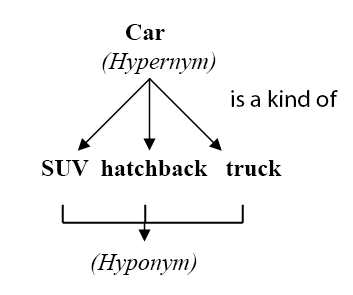
\includegraphics[scale=0.33]{img/wordnet_hyp.png}
\end{minipage}
% This relation is transitive so if for example a car is a kind of vehicle then a truck is also a kind of vehicle. Reaction time word association experiments with humans suggest that knowledge is stored in the brain at superordinate nodes and inherited downward. 
\end{frame}

\begin{frame}
\frametitle{Meronym / Holonym (part/whole)}
\begin{minipage}{0.5\textwidth}
\begin{itemize}
\item The engine (Hyponym) is a part of a car (Hypernym)
\item denotes more or less general concepts
\item inheritance
\item 3 kinds of meronomy
\begin{itemize}
\item proper parts
\item substance
\item groups/members
\end{itemize}
\end{itemize}
\end{minipage}
\begin{minipage}{0.4\textwidth}
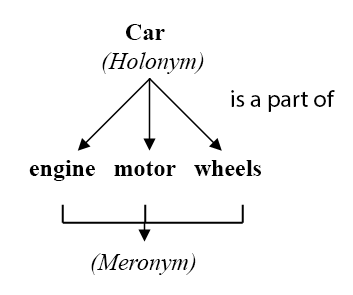
\includegraphics[scale=0.33]{img/wordnet_mer.png}
\end{minipage}
% An example for the inheritance would be that is an engine has spark plugs and an enginge is part of a car, then a car also has spark plugs. 
% WordNet distinguishes between 3 different kinds of Meronomy. First there are proper parts, which are seperable, like in the example: car - engine, or motor engine. Then there is are substances such as oxygen which is a part of air and water and members of groups like professor and faculty.
\end{frame}

\begin{frame}
\frametitle{Semantic Relations between Verbs}
\begin{itemize}
\item apart from Homonyms
\begin{itemize}
\item Troponym:\\
the verb Y is a troponym of the verb X if the activity Y is doing X in some manner (lisp- talk)
\item Entailment:\\
the verb Y is entailed by X if by doing X you must be doing Y (sleep - snore)
\end{itemize}
\end{itemize}
%the verb Y is a troponym of the verb X if the activity Y is doing X in some manner (to lisp is a troponym of to talk)
%the verb Y is entailed by X if by doing X you must be doing Y (to sleep is entailed by to snore)
\end{frame}

\begin{frame}
\frametitle{Problems and Limitations}
\begin{itemize}
\item doesn't contain etymology, pronunciation or irregular verbs
\item hard to modify or maintain
\item no special domain vocabulary
\item granularity
\end{itemize}
\end{frame}


\begin{frame}
\frametitle{Demo}
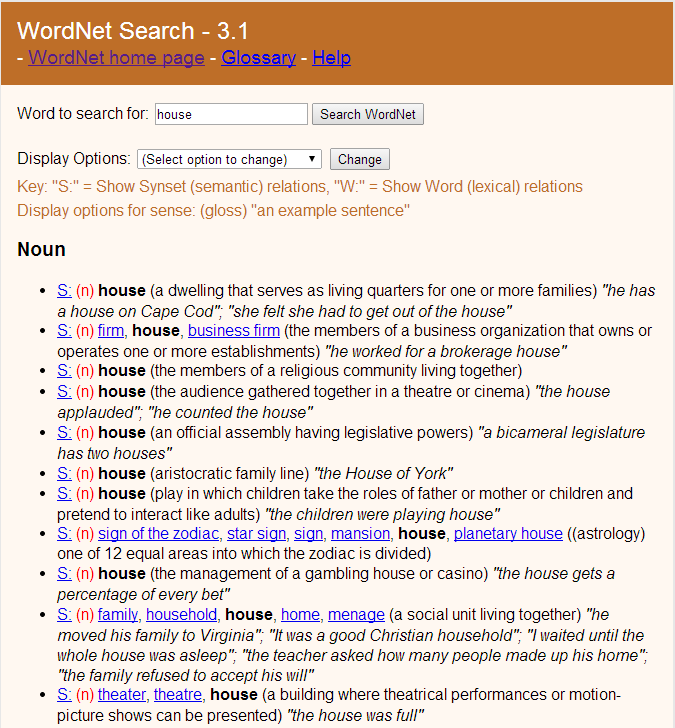
\includegraphics[scale=0.29]{img/wordnet_demo.png}\\
http://wordnetweb.princeton.edu/perl/webwn
\end{frame}

\begin{frame}
\frametitle{Application}
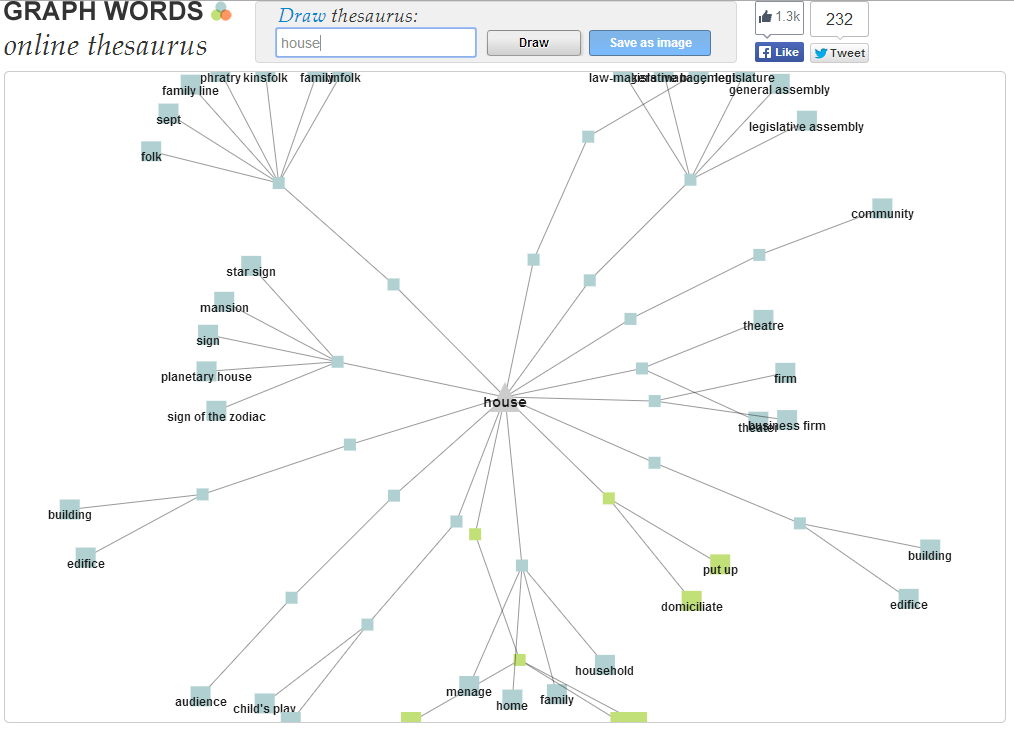
\includegraphics[scale=0.29]{img/wordnet_app.png}\\
http://graphwords.com/
\end{frame}

\begin{frame}
\frametitle{Other WordNets}
There are many other WordNets for other languages
\begin{itemize}
\item Universal WordNet
\begin{itemize}
\item 1.5 million words
\item 200 languages
\item based on WordNet
\item MENTA integration\\
$\rightarrow$15 million words and names
\end{itemize}
\end{itemize}
\end{frame}
	
	

\section{Yago}
\begin{frame}
\frametitle{YAGO Yet Another Great Ontology}

\includegraphics[scale=0.25]{img/yago_logo_small.png}
\begin{itemize}
\item YAGO (2008) YAGO2s (2012)
\item developed at Max Planck Institute for Computer Science
\item more than 10 million entities
\item more than 447 million facts
\end{itemize}
%YAGO in its newest Version YAGO2s is a very big knowledgebase developed at the Max Planck Institute for Computer Science. In 2012, YAGO2s had knowledge of more than 10 million entities and contained more than 120 million facts about these entities.
\end{frame}

\begin{frame}
\frametitle{Extraction from:}

\includegraphics[scale=0.31]{img/yago-figure2.png}
%These are exclusively extracted from: Wikipedia, WordNet, GeoNames, WordNet Domains (,which augments WordNet with domain labels) and the Universal WordNet (which is the multilingual approach on WordNet).\\
\end{frame}

\begin{frame}
\frametitle{Extracts from Wikipedia:}
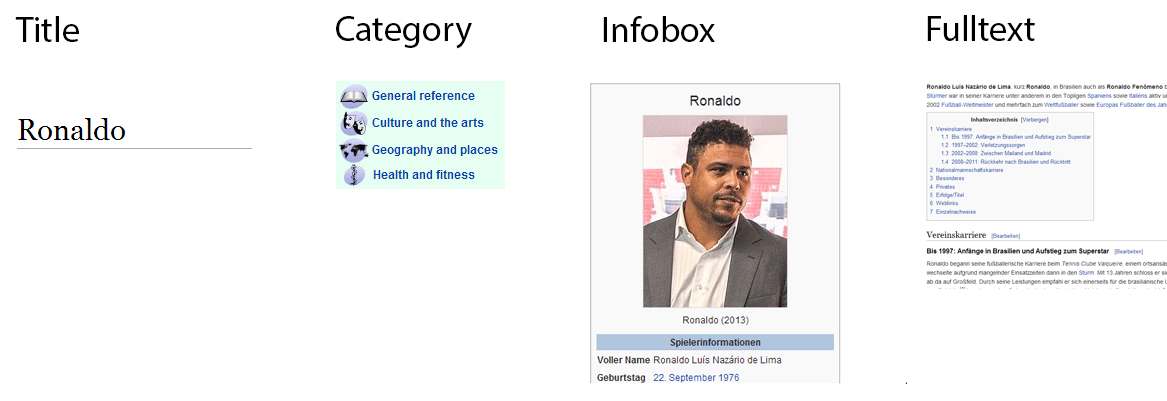
\includegraphics[scale=0.25]{img/yago-figure3.png}
%Now we have already one big knowledge-base which is extractin from Wikipedia, DBpedia, why do we need YAGO. Well, for one YAGO extracts the infoboxes, categories and fulltext, whereas DBPedia mainly takes facts from the infoboxes.
\end{frame}

\begin{frame}[fragile]
\frametitle{Relations:}
\begin{itemize}
\item YAGO:\\
about predefined relations with domain and range:\\
\begin{lstlisting}[frame=single]
:hasSon rdfs:domain :Person;
            rdfs:range  :Man.
\end{lstlisting}
adds temporal and spatial dimension to many entities/relations
\item DBpedia:\\
used to use words from infoboxes\\
$\rightarrow$ length, length-in-km, length-km
now uses also predefined relations
\end{itemize}
%Then YAGO has about 100 manually predefined relations with domains and ranges, while DBPedia used to use the words it finds in the infoboxes. As a drawback the same relation may appear with different names. In the meantime DBpedia updated its process and uses also predefined relations.
\end{frame}

\begin{frame}[fragile]
\frametitle{Relations: Time and Space}
\begin{itemize}
\item many facts have a spatial and temporal dimension
\begin{itemize}
\item Josef Ackermann is CEO of Deutsche Bank (2006-2012, London)
\end{itemize}
\item not covered by rdf and SPARQL
\item triplets to 5-lets
\item SPARQL to SPOTL(X)
\item still RDF
\end{itemize}
%Many facts have  also a spatial and temporal domain. For example the fact "Josef Ackermann is CEO of Deutsche" Bank is not valid today, because it also has a time domain. He was in fact CEO of Deustche Bank but only from 2006 to 2012. This kind of additional information can not be stored in traditional RDF that is why RDF facts in Yago also have the information about time and space in form from comments. This way normal rdf reader can still use the facts but more sophisticated extractors can use the additional information.
\end{frame}

\begin{frame}
\frametitle{Demo spotlx}
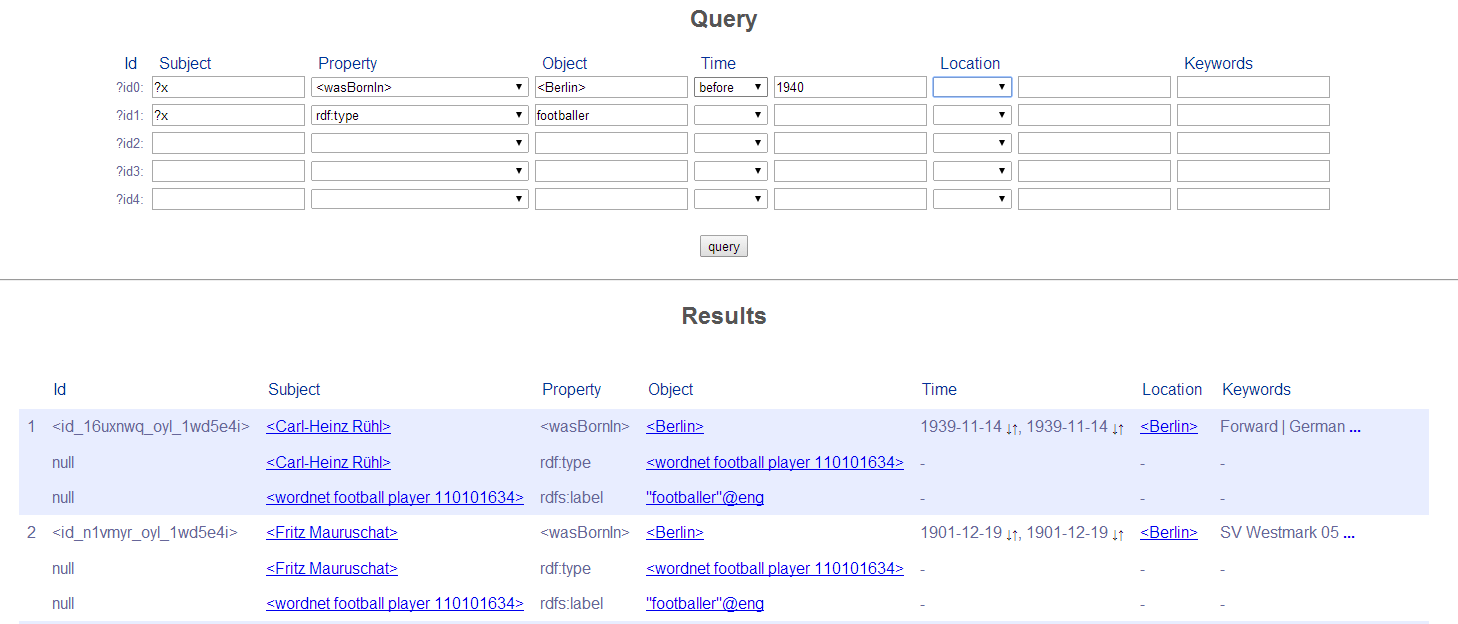
\includegraphics[scale=0.2]{img/yago-spotnx.png}\\
https://gate.d5.mpi-inf.mpg.de/webyagospotlx/WebInterface
\end{frame}

\begin{frame}
\frametitle{Precision and costs}
\begin{itemize}
\item YAGO:
\begin{itemize}
\item manually evaluated that 95% triplets are correct
\item extractions process lasts 3 days
\item over 12 researcher
\end{itemize}
\end{itemize}
%All this make YAGO a very precise database. A manual evaluation confirmed that 95\% of the triplets extracted by YAGO are correct. But this comes at the price of speed and maintenance. Because YAGO draws from few but very different sources, the extraction, reconciliation, deduplication, verification of constraints, etc. takes several days to run. Plus more than a dozen researches, who need to work directly or indirectly on YAGO.\\
\end{frame}

\begin{frame}
\frametitle{Why YAGO?}
\begin{tabular}{l|c|r}
& YAGO & DBpedia\\
\hline 
extracts: & title, category, infobox, fulltext & mainly infobox\\
relations: & predefined (domain, range) & taken from infobox\\
precision: & very good & not that good \\
costs: & very high & not that high

% Here we see again a direct comparision between YAGO and DBpedia
\end{tabular}
\end{frame}

\begin{frame}
\frametitle{Extraction-process and Sources}
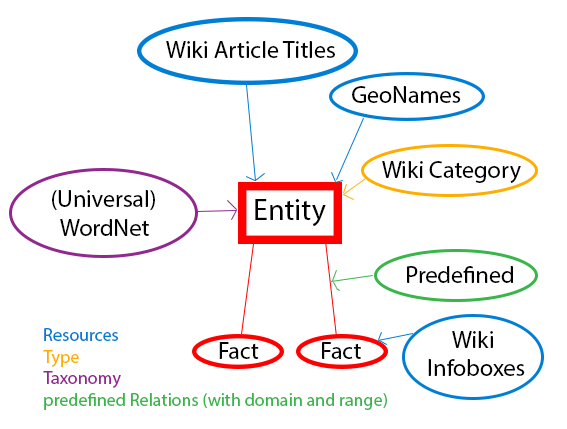
\includegraphics[scale=0.35]{img/yago-ex1.png}
%The extraction of the original YAGO looks like this. The titles of the Wikipedia articles contribute the entities. The wikipedia-categories are analyzed to derive the entities type. Then the infoboxes are extracted to get facts about the entity, which are stored in predefined relations. WordNet and Universal WordNet deliver the taxonomic backboneand then GeoNames is used to merge additional Entities into the ontology.
\end{frame}

\begin{frame}
\frametitle{YAGO2s}
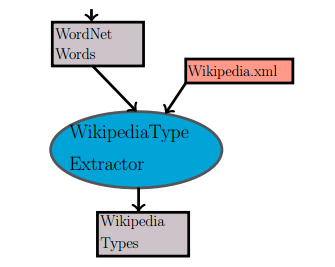
\includegraphics[scale=0.7]{img/yago_figure.PNG}
%YAGO2s introduced a transparent and modular architecture. Main ingredients are themes and extractors.\\
%A theme, represented by these rectangles, is a collection of facts, such as all facts derived from WordNet, or facts concerning people. These facts are completely RDF compliant and stored in turtle format with additional fact identifiers to integrate time and space information. \\
%Then we have extractors, these ellipses. Extractors have a number themes as input and a number of themes as output. Such as an extractor for deduplication which takes a number of themes as input and puts a deduplicated theme out. Then there are also Extractors which can take external data sources as input, represented as these smaller rectangles. For example the Wikipedia Category Extractor, which takes Wikipedias XML-dump as input and produces a theme with facts extracted from Wikipedia-categories.\\
\end{frame}

\begin{frame}
\frametitle{Visualization}
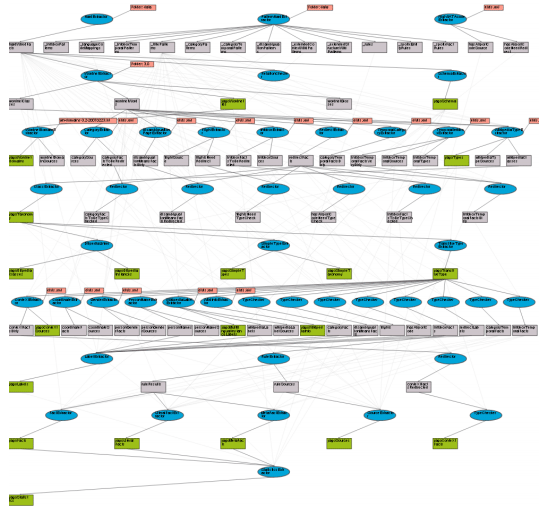
\includegraphics[scale=0.32]{img/yago_visual.png}\\
http://resources.mpi-inf.mpg.de/yago-naga/yago/www2013demo/yago\_demo\_static/
%This is a visualization of all these extractors and themes as a dependency graph. It also integrates the scheduling constraints of YAGO. Some extractors have to be executed in a certain order and some can be executed in parallel. The lines show which extractor rpodues which theme and which theme is used by which extractor. We can see four main types of extractors: Wikipedia extractors which are exclusively concerned with Wikipedia-sources, GeoNames which harvest and map entities from GeoNames, External extractors which extract from (Universal) WordNet and WordNet domains and Theme Extractors which exclusively take Themes as input, such as the deduplicator or a constraints checker. Some extractors, for example the Type Checker, are instantiated multiple time, so that the overall amount of extractors in this visualization rises from 30 unique to 42 extractors.\\
%Another interesting extractor would be the WordNet domains extractor which enriches the entities with domains such as "law" or "music". This enable you to ask for all entities which are related to "music" for example.
\end{frame}

\begin{frame}
\frametitle{Demo Ontology Browser}
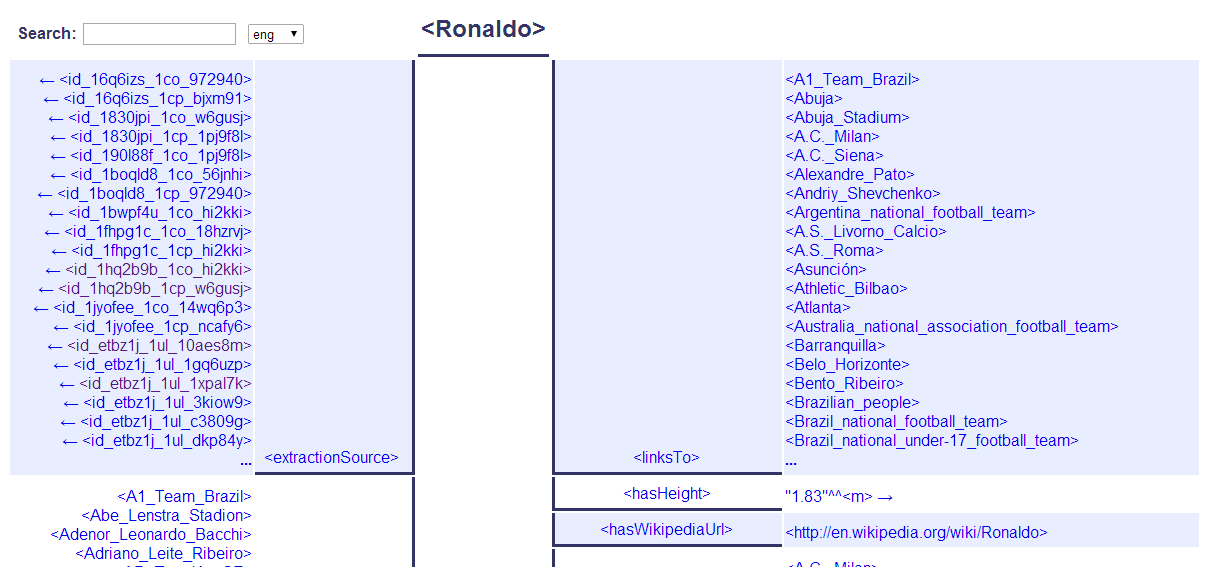
\includegraphics[scale=0.2]{img/yago-obr.png}\\
https://gate.d5.mpi-inf.mpg.de/webyagospotlx/Browser
\end{frame}

\begin{frame}
\frametitle{When to use YAGO}
\begin{itemize}
\item main goal\\
near human-accuracy
\item advantages
\begin{itemize}
\item accuracy
\item coverage by GeoNames and WordNet
\item additional spatial and time domain \\
space: 30 million, time 17 million
\end{itemize}
\item disadvatages
\begin{itemize}
\item hard to maintain/ not that up-to-date
\item not many and unreliable SPARQL/ SPOTL(x) endpoints
\end{itemize}
\end{itemize}
\end{frame}


	
	\section{DBpedia}
 
	\section{Freebase}

\begin{frame}
\frametitle{Freebase}

\begin{minipage}{0.55\textwidth}

\begin{itemize}
  \item Initiated by Metaweb in 2007 (Google since 2010)
  \item User for Google Web/Knowledgegraph
  \item Graph based knowledge base
  \item Information is supplied directly by users or automatically through
  specific data pipelines (Wikipedia and Netflix)
\end{itemize}
\end{minipage}
\hfill %wichtig, hier keine leerzeile im code
\begin{minipage}{0.35\textwidth}
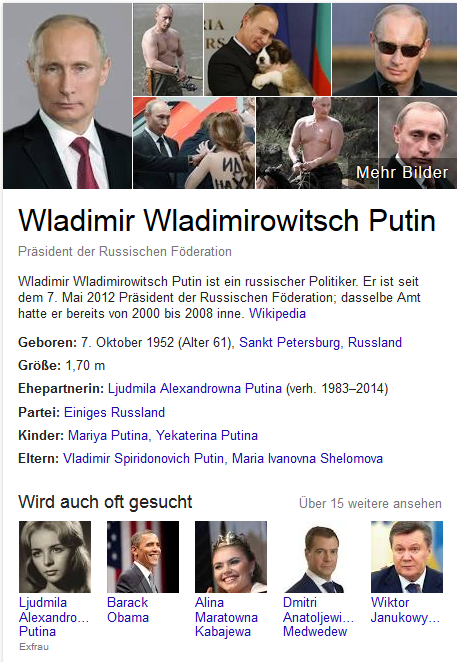
\includegraphics[scale=0.25]{img/putin_freebase.png}
\end{minipage}
\end{frame}

\begin{frame}
\frametitle{Concepts}
\begin{itemize}
  \item Topics = nodes of the graph (Bob Dylan, Mercedes, \ldots)
  \item Properties = edges of the graph (born in, produces, \ldots)
  \item Type (songwriter, actor, car, \ldots)
  \begin{itemize}
    \item Compound Value Types
   \end{itemize}
  \item Domain (music, business, \ldots)
  \item Hierarchical URIs (e.g.
  \url{http://www.freebase.com/} \\ \url{automotive/engine/horsepower})
\end{itemize}
\end{frame}

\begin{frame}
\frametitle{Access}
 Read
  \begin{itemize}
  \item RDF API
  \begin{itemize}
    \item  \url{http://rdf.freebase.com/ns/en.al_gore}
  \end{itemize}
  \item Search API (text search, ordered results after relevance)
  \begin{itemize}
    \item  \url{www.googleapis.com/freebase/v1/search?query=gore}
  \end{itemize}
  \item Topic API (get the JSON for a specific topic)
  \begin{itemize}
    \item  \url{www.googleapis.com/freebase/v1/topic/en/al_gore}
  \end{itemize}
  \item Data dumps
  \item Freebase Search Widget (jQuery plugin)
  \end{itemize}
  Read/Write
  \begin{itemize}
  \item MQL API
  \item Webpage (edit data, create views)
  \end{itemize}
  The Google APIs are available for Java, PHP, Python, .NET, JavaScript,
  Objective-C
\end{frame}

\begin{frame}[fragile]
\frametitle{Metaweb Query Language}
\begin{itemize}
  \item Read request sends and gets JSON
  \item[]
  \item
  \url{https://www.googleapis.com/freebase/v1/mqlread?query=\_jsonInput\_}\\
    \begin{verbatim}_jsonInput_:= {"type":"/music/artist",
  	            "name":"The Police",
  	            "album":[]}} 
\end{verbatim}
\end{itemize}
\end{frame}



\begin{frame}[fragile]
\frametitle{Metaweb Query Language}
\begin{itemize}
  \item Write request sends and gets JSON
  \item[]
  \item
  \url{https://www.googleapis.com/freebase/v1sandbox/mqlwrite?oauth_token=_token_&query=_query_}\\
    \begin{verbatim}_query_:= {"create":"unconditional",
		           "id":null,
		           "name":"Nowhere",
		           "type":"/location/location"} 
\end{verbatim}
\end{itemize}
\end{frame}
	
	
	\begin{frame}
	\frametitle{comparison}
	\begin{table}
	\begin{tabular}{|l|l|l|}
	\hline
	 & DBpedia & Freebase\\
	 Sources & only Wikipedia & Wikipedia, Netflix, user input\\
	 $+$ & \parbox[t]{4cm}{has many outgoing links\\ good categorization} & 
	 \parbox[t]{5cm}{many sources\\possibly more information}\\
	 $-$ & limited information & \parbox[t]{5cm}{might seem a bit\\unstructured at
	 times \\ no SPARQL endpoint} \\
	\hline
	\end{tabular}
	\end{table}
	\end{frame}
	
	\begin{frame}
	\frametitle{comparison}
	\begin{table}
	\begin{tabular}{|l|l|l|}
	\hline
	 & WordNet & YAGO\\
	 Sources & manual & \parbox[t]{4cm}{Wikipedia, GeoNames, WordNet\\ Universal WordNet}\\
	 $+$ & \parbox[t]{3.2cm}{good for word sense\\ disambiguation\\ really big} & 
	 \parbox[t]{4cm}{additional spatial and temporal information\\ many sources\\very precise}\\
	 $-$ & \parbox[t]{3.2cm}{too fine-grained\\ no domain-specific\\ vocabulary} & \parbox[t]{4cm}{not that up-to-date \\ no good SPARQL endpoint} \\
	\hline
	\end{tabular}
	\end{table}
	\end{frame}
	
	
\end{document}